\subsection{Experimental Evaluation}
\label{sec:exp}

Next, we report results from a comprehensive evaluation of our methods against real-world datasets.

\subsubsection{Experimental Setup}
\label{subsec:evaluation_setup}

\vspace{2mm}

\subsubsubsection{Datasets}
We use three real-world datasets (Table \ref{tab:datasets}) selected from different application domains, containing diverse types of geolocated time series, as detailed below:

\begin{table}[t]
	\centering
	\caption{Datasets and parameters used in the experiments.}
	\vspace{-10pt}
	\begin{small}
	\centering
	\resizebox{\linewidth}{!}{%
	\begin{tabular}{lccc|cccc}
	\hline
	\multirow{2}{*}{Dataset} & Area & Number of & Length of & \multicolumn{4}{c}{Default query parameters} \\
	 & (km$^2$) & locations & timeseries & $\rho$ & $\epsilon$ & $\delta$ & $k$ \\
	\hline
	Flickr & Earth & 414,967 & 96 & 30\% & 7.5\% & 20 & 30\\
    Crime & 392,000 & 362,215 & 76 & 30\% & 7.5\% & 25 & 30 \\
    Taxi & 2,500 & 417,960 & 168 & 30\% & 10\% & 20 & 30 \\
	\hline
	\end{tabular}}
	\end{small}
	\label{tab:datasets}
\end{table}

\vspace{2mm}

\noindent \emph{\textbf{UK historical crime data (Crime)}}. Contains time series representing the temporal variation in the number of crime incidents reported across England and Wales over 76 months (December 2010-- March 2017). We generated time series over a grid with cell size 200 meters applied on the original data\footnote{\url{https://data.police.uk/data/}}. For each month, we counted incidents having their location within each cell.

\vspace{2mm}

\noindent \emph{\textbf{Flickr geotagged photos (Flickr)}}. Contains time series data extracted from geolocated Flickr images between 2006 and 2013 over the entire planet\footnote{\url{https://code.flickr.net/category/geo/}}. To get meaningful geolocated time series, we partitioned the space by a uniform grid of of $7200 \times 3600$ cells (each one spanning $0.05$ decimal degrees in each dimension) and counted the number of photos contained in every cell each month. We excluded empty cells (e.g., in the oceans). Each time series conveys the visits pattern (in terms of number of photos taken per month) of that region over this period.

\vspace{2mm}

\noindent \emph{\textbf{NYC taxi dropoffs (Taxi)}}. Contains time series extracted from yellow taxi rides in New York City during 2015. The original data\footnote{\url{http://www.nyc.gov/html/tlc/html/about/trip_record_data.shtml}} provide pick-up and drop-off locations, as well as corresponding timestamps for each ride. For each month, we generated time series by applying a uniform spatial grid over the entire city (cell side was 200 meters) and counting all drop-offs therein for each day of the week at the time granularity of one hour. Thus, we obtained the number of drop-offs for $24 \times 7$ time intervals in every cell, which essentially captures the weekly fluctuation of taxi destinations there. Without loss of generality, the centroid of each cell is used as the geolocation of the corresponding time series. 

\vspace{2mm}

\noindent \emph{\textbf{Synthetic}}. To test scalability, we augmented the Flickr dataset by slightly moving each location in a random manner and altering each time series value by a random number between $1$ and $10$. We produced three additional synthetic datasets each containing $\times 2$, $\times 3$, $\times 4$ the number of time series from the original dataset. 

%(i.e., 829,934, 1,244,901 and 1,659,868).

\subsubsubsection{Index and Query Parameters}
To evaluate the performance benefits observed in the experiments only based on pruning, we tuned the index parameters to fixed values. The minimum ($m$) and maximum ($M$) number of entries stored in each node are set to $40$ and $100$, respectively. For both \btsr and \sbtsr, the number of MBTS to 10 and for \sbtsr, the number of segments $s$ is also set to 10. The query parameters involve the spatial distance and local similarity thresholds, i.e., $\rho$, $\epsilon$, $\delta$ and $k$. The values of these parameters are set differently for each dataset, based on their characteristics; default values are shown in Table \ref{tab:datasets}. The value of $\rho$ is set relatively, by setting the covered area as a percentage of the total area. Similarly, $\epsilon$ is set as a percentage of the maximum difference between the observed values.

\subsubsubsection{Evaluation Setting}
%We compare the performance of $\mathcal{S}$BTSR-\\Tree against the checkpoint-based and sweep line-based \btsr. 
Each experiment is performed using a randomly selected workload of 100 queries for each dataset and we report the average response time. All indices are held in memory, while the leafs contain pointers to files with geolocated time series stored on disk. All methods were developed in Java. Tests were executed on a server with 4 CPUs, each containing 8 cores clocked at 2.13GHz, and 256 GB RAM running Debian Linux.

\subsubsection{Query Performance}
\label{subsec:query_perf}

We compare the average per query execution time for all three queries using sweep line and checkpoint methods on \btsr and the checkpoint method on \sbtsr.

\begin{figure}[htbp]
\subfloat{\fbox{
\includegraphics[width=0.35\textwidth]{Figures/legend.png}}}
\\
\vspace{-5pt}
\subfloat[Crime]{\includegraphics[trim=0.5cm 0.5cm 0.5cm 0.5cm, clip, width=0.225\textwidth]{Figures/Plots/Crime/varying_epsSP.eps}\label{subfig:var_epsSP_crime}} \quad
\subfloat[Crime]{\includegraphics[trim=0.5cm 0.5cm 0.5cm 0.5cm, clip, width=0.225\textwidth]{Figures/Plots/Crime/varying_epsTS.eps}\label{subfig:var_epsTS_crime}} \\
\vspace{-5pt}
\subfloat[Flickr]{\includegraphics[trim=0.5cm 0.5cm 0.5cm 0.5cm, clip, width=0.225\textwidth]{Figures/Plots/Flickr/varying_epsSP.eps}\label{subfig:var_epsSP_flickr}} \quad
\subfloat[Flickr]{\includegraphics[trim=0.5cm 0.5cm 0.5cm 0.5cm, clip, width=0.225\textwidth]{Figures/Plots/Flickr/varying_epsTS.eps}\label{subfig:var_epsTS_flickr}} \\
\vspace{-5pt}
\subfloat[Taxi]{\includegraphics[trim=0.5cm 0.5cm 0.5cm 0.5cm, clip, width=0.225\textwidth]{Figures/Plots/Taxi/varying_epsSP.eps}\label{subfig:var_epsSP_taxi}} \quad
\subfloat[Taxi]{\includegraphics[trim=0.5cm 0.5cm 0.5cm 0.5cm, clip, width=0.225\textwidth]{Figures/Plots/Taxi/varying_epsTS.eps}\label{subfig:var_epsTS_taxi}}
\vspace{-5pt}
\caption{Query $Q_{rr}(T_q, \rho, \epsilon, \delta)$ for varying $\rho$ and $\epsilon$.}
\label{fig:query1a}
\end{figure}

\begin{figure*}[htbp]
\centering
\subfloat{\fbox{
\includegraphics[width=0.35\textwidth]{Figures/legend.png}}}
\\
\vspace{-5pt}
\subfloat[Crime ($Q_{rr}$)]{\includegraphics[trim=0.5cm 0.5cm 0.5cm 0.5cm, clip, width=0.225\textwidth]{Figures/Plots/Crime/varying_delta.eps}\label{subfig:var_delta_crime}}
\subfloat[Crime ($Q_{kr}$)]{\includegraphics[trim=0.5cm 0.5cm 0.5cm 0.5cm, clip, width=0.225\textwidth]{Figures/Plots/Crime/varying_k_query2.eps}\label{subfig:var_k_crime}}
\subfloat[Crime ($Q_{rk}$)]{\includegraphics[trim=0.5cm 0.5cm 0.5cm 0.5cm, clip, width=0.225\textwidth]{Figures/Plots/Crime/varying_k_query3.eps}\label{subfig:var_ks_crime}}
\subfloat[$Q_{rr}$]{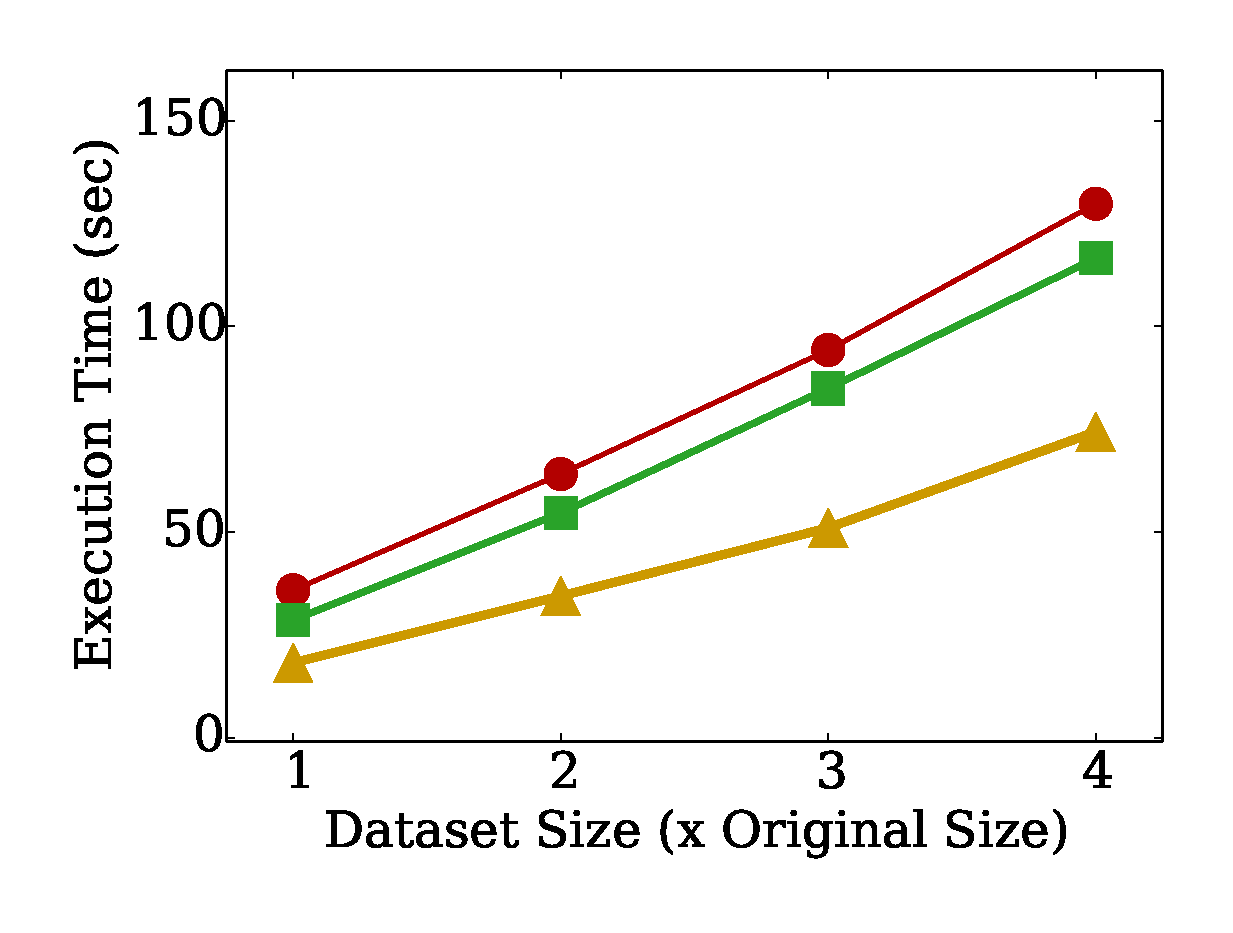
\includegraphics[trim=0.5cm 0.5cm 0.5cm 0.5cm, clip, width=0.225\textwidth]{Figures/Plots/Scalability/varyingDatasetSize_1.eps}\label{subfig:scalability1}} \\
\vspace{-5pt}
\subfloat[Flickr ($Q_{rr}$)]{\includegraphics[trim=0.5cm 0.5cm 0.5cm 0.5cm, clip, width=0.225\textwidth]{Figures/Plots/Flickr/varying_delta.eps}\label{subfig:var_delta_flickr}}
\subfloat[Flickr ($Q_{kr}$)]{\includegraphics[trim=0.5cm 0.5cm 0.5cm 0.5cm, clip, width=0.225\textwidth]{Figures/Plots/Flickr/varying_k_query2.eps}\label{subfig:var_k_flickr}}
\subfloat[Flickr ($Q_{rk}$)]{\includegraphics[trim=0.5cm 0.5cm 0.5cm 0.5cm, clip, width=0.225\textwidth]{Figures/Plots/Flickr/varying_k_query3.eps}\label{subfig:var_ks_flickr}}
\subfloat[$Q_{kr}$]{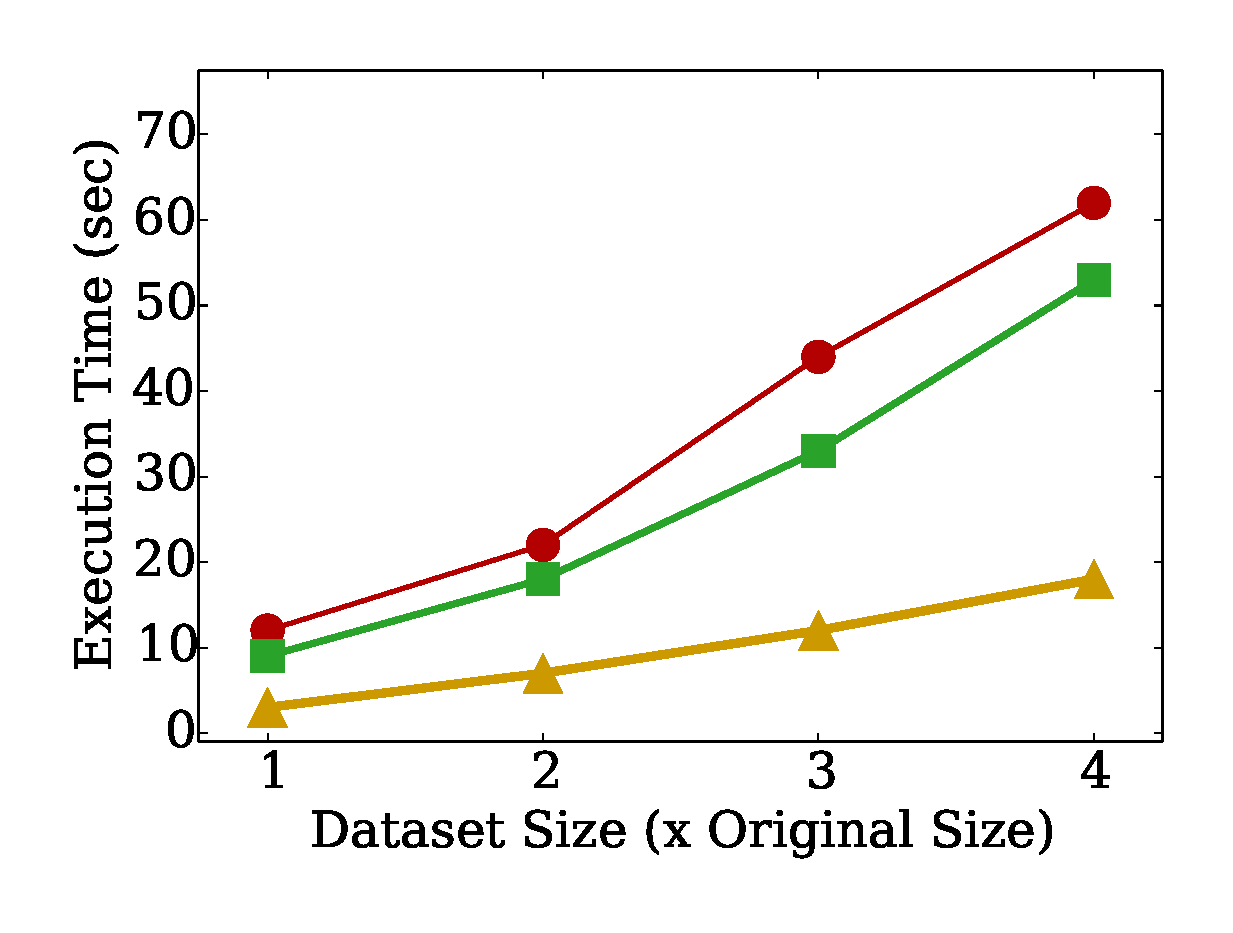
\includegraphics[trim=0.5cm 0.5cm 0.5cm 0.5cm, clip, width=0.225\textwidth]{Figures/Plots/Scalability/varyingDatasetSize_2.eps}\label{subfig:scalability2}} \\
\vspace{-5pt}
\subfloat[Taxi ($Q_{rr}$)]{\includegraphics[trim=0.5cm 0.5cm 0.5cm 0.5cm, clip, width=0.225\textwidth]{Figures/Plots/Taxi/varying_delta.eps}\label{subfig:var_delta_taxi}}
\subfloat[Taxi ($Q_{kr}$)]{\includegraphics[trim=0.5cm 0.5cm 0.5cm 0.5cm, clip, width=0.225\textwidth]{Figures/Plots/Taxi/varying_k_query2.eps}\label{subfig:var_k_taxi}}
\subfloat[Taxi ($Q_{rk}$)]{\includegraphics[trim=0.5cm 0.5cm 0.5cm 0.5cm, clip, width=0.225\textwidth]{Figures/Plots/Taxi/varying_k_query3.eps}\label{subfig:var_ks_taxi}}
\subfloat[$Q_{rk}$]{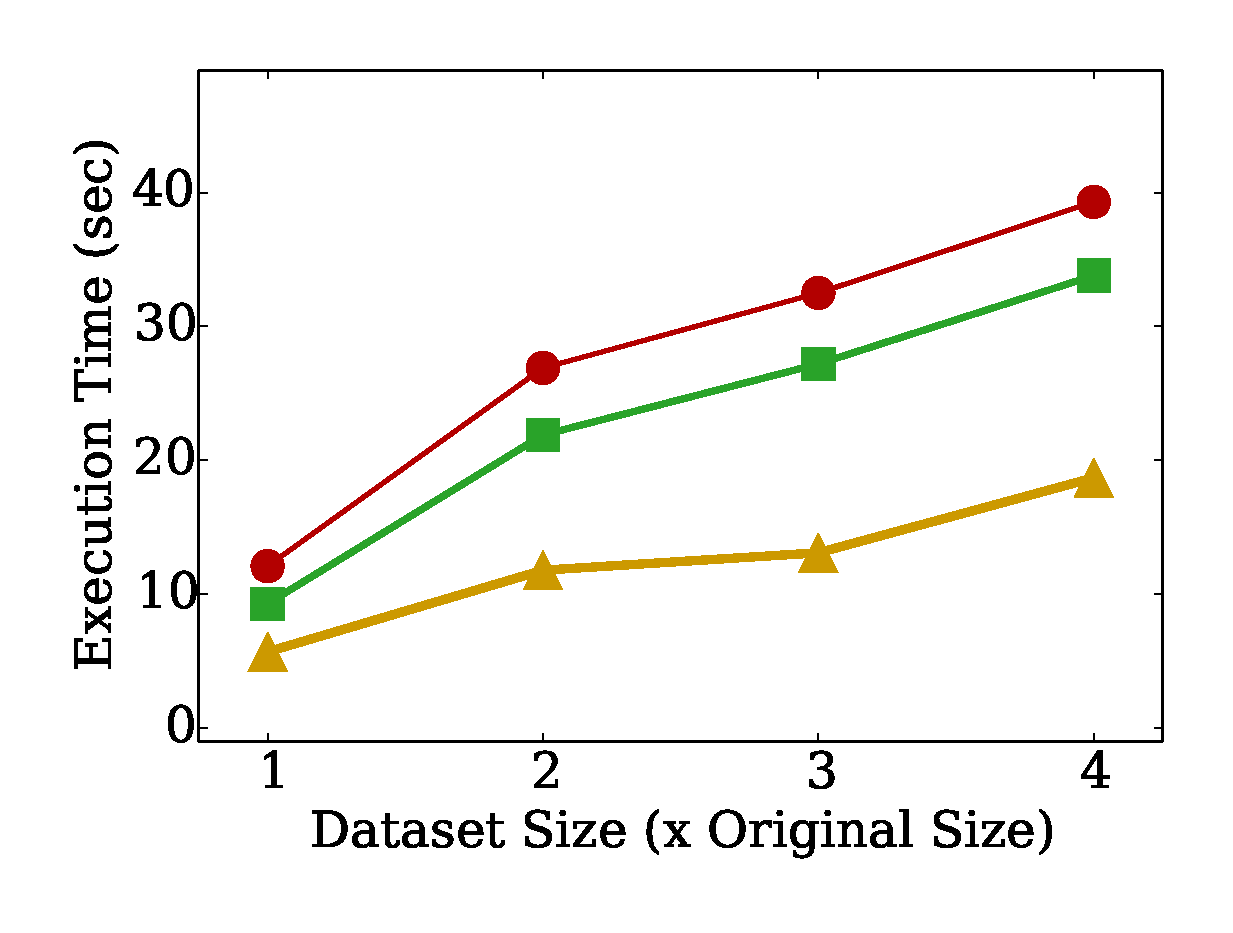
\includegraphics[trim=0.5cm 0.5cm 0.5cm 0.5cm, clip, width=0.225\textwidth]{Figures/Plots/Scalability/varyingDatasetSize_3.eps}\label{subfig:scalability3}}
\vspace{-5pt}
\caption{Per column: $Q_{rr}(T_q, \rho, \epsilon, \delta)$ for varying $\delta$ -- $Q_{kr}(T_q, k, \epsilon, \delta)$ for varying $k$ -- $Q_{rk}(T_q, k, \rho)$ for varying $k$ -- Scalability. }
\label{fig:exp}
\end{figure*}

\subsubsubsection{$Q_{rr}(T_q, \rho, \epsilon, \delta)$}
Figure \ref{fig:query1a} illustrates the query performance for varying thresholds $\rho$ and $\epsilon$ and the first column of Figure \ref{fig:exp} for varying $\delta$, on all three datasets. It is apparent that the \sbtsr with the checkpoint approach outperforms the rest in all cases. Its superior pruning power is attributed to the segmentation, which yields tighter bounds within the nodes and consequently less disk accesses. The sweep line and checkpoint methods over \btsr perform similarly in all cases. Both methods access the same nodes, but the checkpoint approach needs to examine significantly less values across time in order to determine local similarities. However, since all local similarity calculations take place in-memory, computation cost does not make a big difference, compared to the lesser node accesses required with the \sbtsr. 

More specifically, for the {\em crime} dataset, relaxing $\rho$ (Figure \ref{subfig:var_epsSP_crime}) has a negative impact on all three methods as more nodes have to be accessed and pruning depends mostly on the $\epsilon$ value. \sbtsr increasingly outperforms the rest as $\rho$ increases, due to its more aggressive pruning on local similarity. For the case of increasing $\epsilon$ (Figure \ref{subfig:var_epsTS_crime}), the result is the opposite, as this way the parameter is relaxed and more nodes get accessed. For very large $\epsilon$ values, pruning is solely based on spatial distance and all approaches perform similarly. Finally, increasing $\delta$ (Figure \ref{subfig:var_delta_crime}) also increases the difference in performance among the three approaches, while it also reduces the average query response time. This is due to large numbers of subsequences qualifying for small $\delta$ values, resulting in more node accesses. As $\delta$ increases, pruning is more rapidly improved in the case of \sbtsr due to its tighter bounds.

The results are similar but with larger differences for the {\em Flickr} dataset (Figures \ref{subfig:var_epsSP_flickr}, \ref{subfig:var_epsTS_flickr} and \ref{subfig:var_delta_flickr}). Intuitively, the less periodicity in a dataset, the more the benefit from segmentation; if the time series in the dataset exhibit periodicity, the bounds that will occur from applying $k$-means clustering on the whole sequences will be relatively tighter than otherwise. The Flickr dataset, due to its nature, is more random than the crime dataset, which justifies the larger differences. This explanation is also supported by the results for the {\em taxi} dataset, illustrated in Figures \ref{subfig:var_epsSP_crime}, \ref{subfig:var_epsTS_crime} and \ref{subfig:var_delta_crime}. Despite a similar behavior in varying all thresholds, the differences in average query response time among the different approaches are smaller than in the crime and Flickr datasets, due to the high daily periodicity of taxi drop-offs.

% \begin{figure}[htbp]
% \centering
% \subfigure[Crime]{\includegraphics[trim=0.5cm 0.5cm 0.5cm 0.5cm, clip, width=0.225\textwidth]{Figures/Plots/Crime/varying_delta.eps}\label{subfig:var_delta_crime}} \quad
% \subfigure[Flickr]{\includegraphics[trim=0.5cm 0.5cm 0.5cm 0.5cm, clip, width=0.225\textwidth]{Figures/Plots/Flickr/varying_delta.eps}\label{subfig:var_delta_flickr}}
% \medskip
% \subfigure[Taxi]{\includegraphics[trim=0.5cm 0.5cm 0.5cm 0.5cm, clip, width=0.225\textwidth]{Figures/Plots/Taxi/varying_delta.eps}\label{subfig:var_delta_taxi}}
% \vspace{-5pt}
% \caption{$Q_{rr}(T_q, \rho, \epsilon, \delta)$ for varying $\delta$. }
% \label{fig:query1b}
% \end{figure}

\subsubsubsection{$Q_{kr}(T_q, k, \epsilon, \delta)$}
Figures \ref{subfig:var_k_crime}, \ref{subfig:var_k_flickr} and \ref{subfig:var_k_taxi} depict the results for the $Q_{kr}(T_q, k, \epsilon, \delta)$ query for the three datasets. As $k$ increases, more nodes have to be traversed in order to fetch the additional results, and the execution time increases for all methods. Nevertheless, \sbtsr still clearly outperforms the other two algorithms.
% \checknote{Similarly to the above observation, the \sbtsr in the taxi dataset offers less benefits compared to the crime and Flickr datasets, for the same reasons.}

% \begin{figure}[htbp]
% \centering
% \subfigure[Crime ($Q_{kr}$)]{\includegraphics[trim=0.5cm 0.5cm 0.5cm 0.5cm, clip, width=0.225\textwidth]{Figures/Plots/Crime/varying_k_query2.eps}\label{subfig:var_k_crime}} \quad
% \subfigure[Crime ($Q_{rk}$)]{\includegraphics[trim=0.5cm 0.5cm 0.5cm 0.5cm, clip, width=0.225\textwidth]{Figures/Plots/Crime/varying_k_query3.eps}\label{subfig:var_ks_crime}}
% \medskip
% \subfigure[Flickr ($Q_{kr}$)]{\includegraphics[trim=0.5cm 0.5cm 0.5cm 0.5cm, clip, width=0.225\textwidth]{Figures/Plots/Flickr/varying_k_query2.eps}\label{subfig:var_k_flickr}} \quad
% \subfigure[Flickr ($Q_{rk}$)]{\includegraphics[trim=0.5cm 0.5cm 0.5cm 0.5cm, clip, width=0.225\textwidth]{Figures/Plots/Flickr/varying_k_query3.eps}\label{subfig:var_ks_flickr}}
% \medskip
% \subfigure[Taxi ($Q_{kr}$)]{\includegraphics[trim=0.5cm 0.5cm 0.5cm 0.5cm, clip, width=0.225\textwidth]{Figures/Plots/Taxi/varying_k_query2.eps}\label{subfig:var_k_taxi}} \quad
% \subfigure[Taxi ($Q_{rk}$)]{\includegraphics[trim=0.5cm 0.5cm 0.5cm 0.5cm, clip, width=0.225\textwidth]{Figures/Plots/Taxi/varying_k_query3.eps}\label{subfig:var_ks_taxi}}
% \vspace{-5pt}
% \caption{$Q_{kr}(T_q, k, \epsilon, \delta)$ and $Q_{rk}(T_q, k, \rho)$ for varying $k$.}
% \label{fig:query2_3}
% \end{figure}

\subsubsubsection{$Q_{rk}(T_q, k, \rho)$}
Finally, Figures \ref{subfig:var_ks_crime}, \ref{subfig:var_ks_flickr} and \ref{subfig:var_ks_taxi} depict the results for the $Q_{rk}(T_q, k, \rho)$ query. In this case, the performance deterioration as $k$ increases is less abrupt, especially for the crime dataset, as usually the top-$k$ results are spatially closely located and are retrieved quickly. Again, the largest and smallest differences are spotted on the Flickr and taxi datasets, respectively.

\subsubsection{Scalability}
\label{subsec:scalability}
We performed a scalability evaluation for all three queries using the Flickr-based synthetic datasets, again measuring the average query response time for the same query workload. The results for increasing dataset size (up to four times) are depicted in Figure \ref{fig:exp}. In all cases, the \sbtsr-based approach scales better, especially in the top-$k$ queries (Figures \ref{subfig:scalability2} and \ref{subfig:scalability3}), where the larger difference observed in Figures \ref{subfig:var_k_flickr} and \ref{subfig:var_ks_flickr} is further augmented.

% \begin{figure}[htbp]
% \centering
% \subfigure[$Q_{rr}(T_q, \rho, \epsilon, \delta)$]{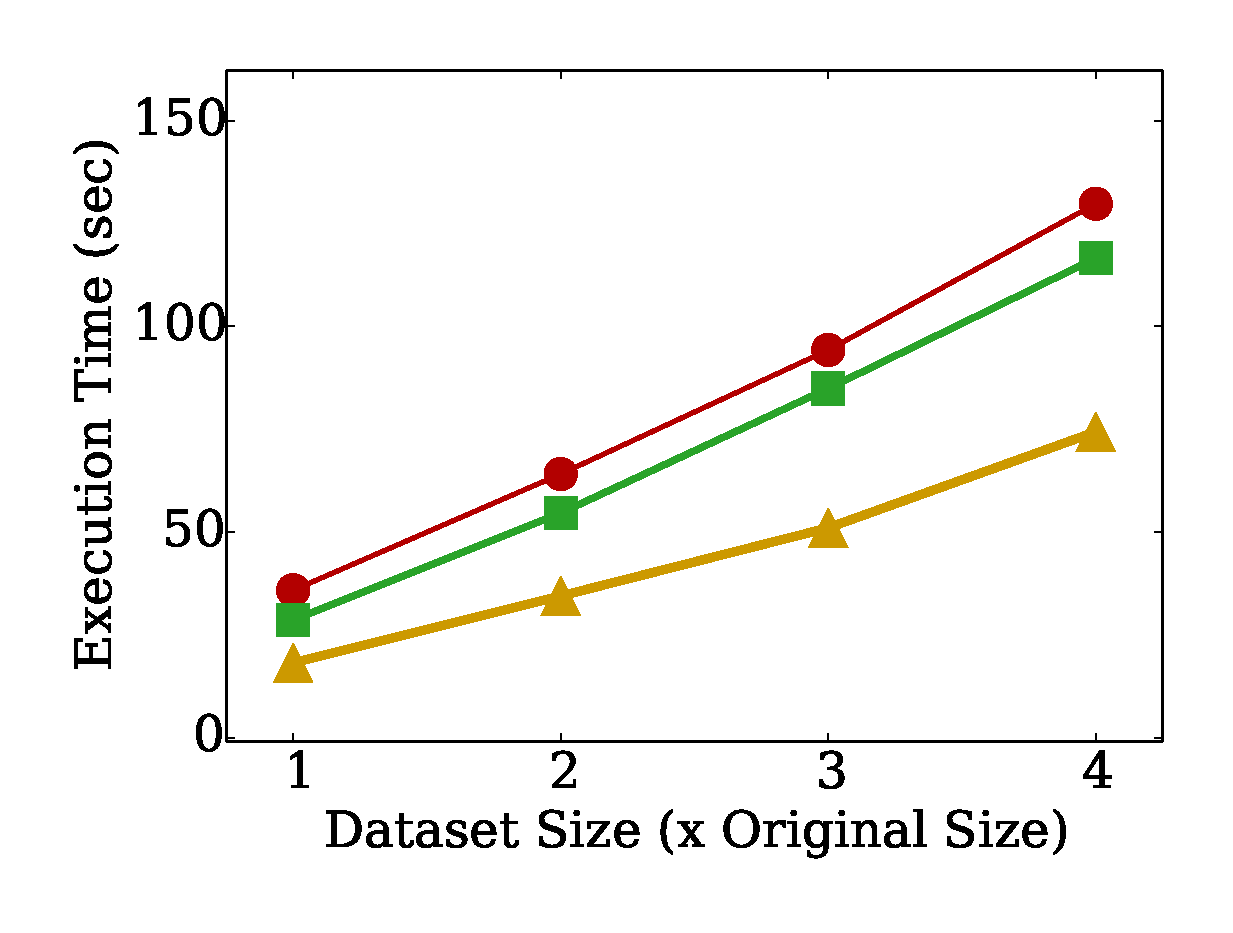
\includegraphics[trim=0.5cm 0.5cm 0.5cm 0.5cm, clip, width=0.225\textwidth]{Figures/Plots/Scalability/varyingDatasetSize_1.eps}\label{subfig:scalability1}} \quad
% \subfigure[$Q_{kr}(T_q, k, \epsilon, \delta)$]{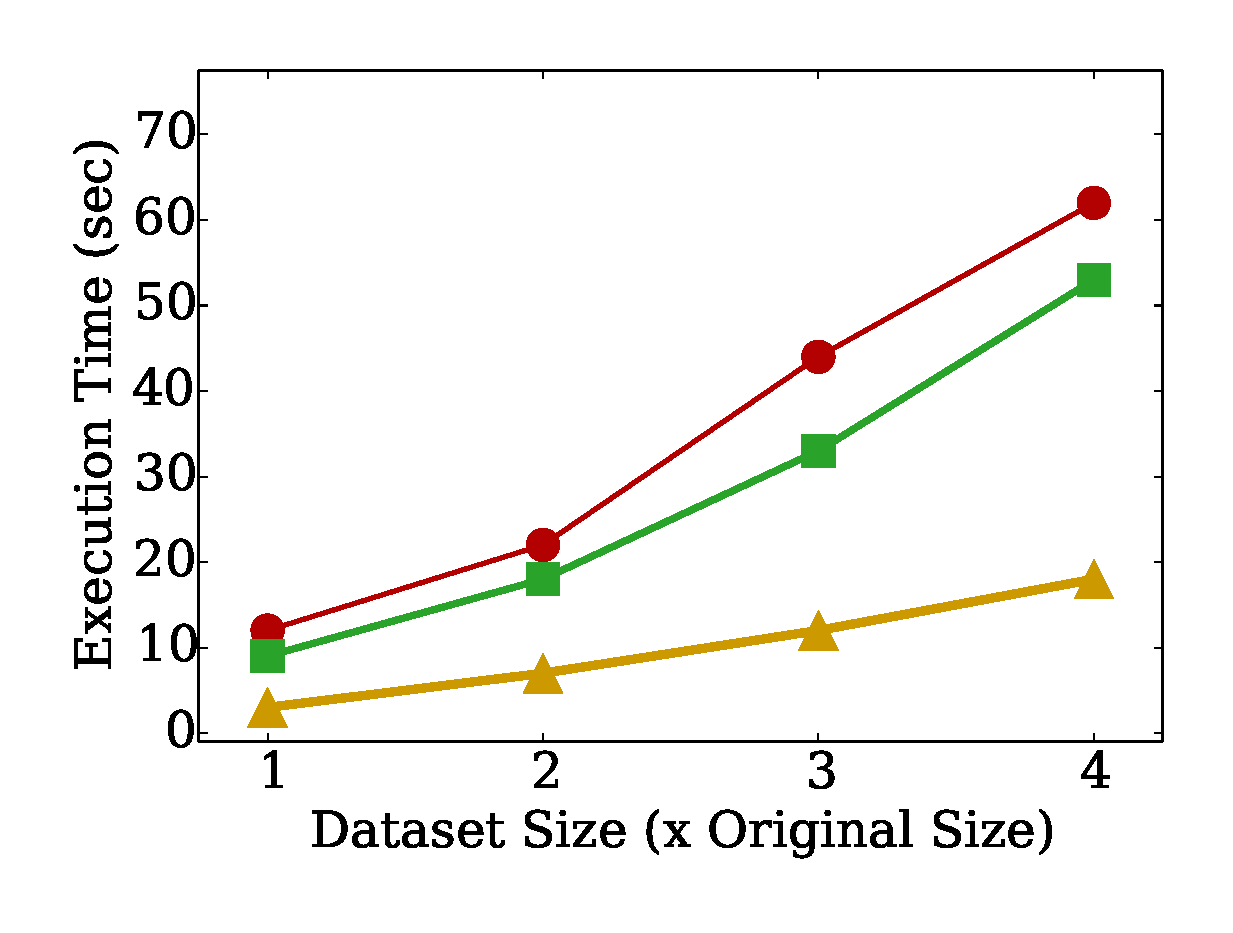
\includegraphics[trim=0.5cm 0.5cm 0.5cm 0.5cm, clip, width=0.225\textwidth]{Figures/Plots/Scalability/varyingDatasetSize_2.eps}\label{subfig:scalability2}}
% \medskip
% \subfigure[$Q_{rk}(T_q, k, \rho)$]{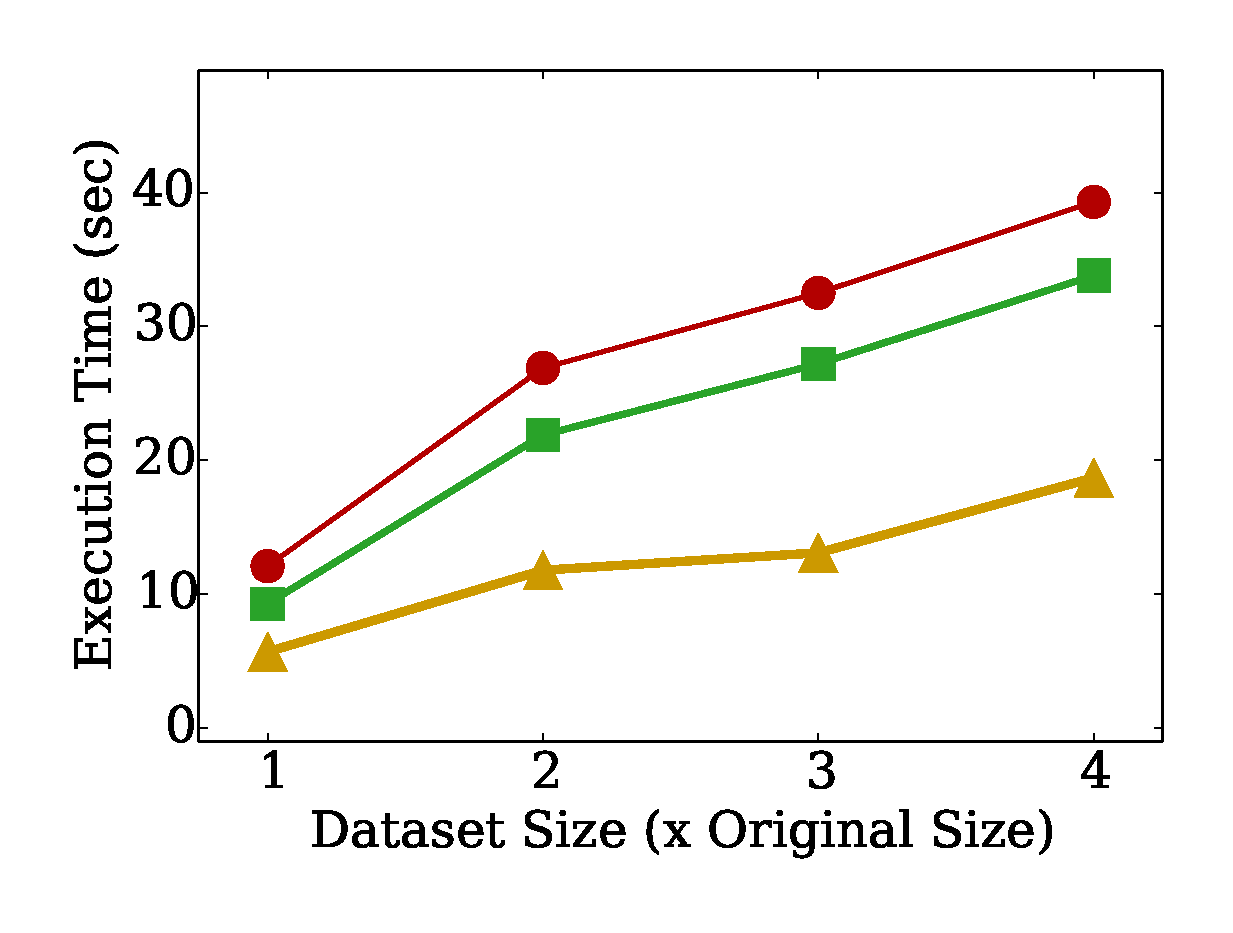
\includegraphics[trim=0.5cm 0.5cm 0.5cm 0.5cm, clip, width=0.225\textwidth]{Figures/Plots/Scalability/varyingDatasetSize_3.eps}\label{subfig:scalability3}}
% \vspace{-5pt}
% \caption{All queries for varying dataset size.}
% \label{fig:scalability}
% \end{figure}